\documentclass[11pt]{article}
\usepackage[table]{xcolor}
\usepackage{amsmath} 
\usepackage{graphicx}
\usepackage{subcaption}
\usepackage{sectsty}
\usepackage{amssymb}
 \usepackage{lipsum}
\usepackage{titlesec}
\usepackage{romannum}
\usepackage{enumitem}
\usepackage{mathtools}
\usepackage[super]{nth}
\usepackage{tikz}
\usepackage{listings}
\usepackage{pagecolor,lipsum}
\usepackage{color,soul}
\usepackage{xcolor}
\usepackage{hyperref}
\usepackage[T1]{fontenc}
\usepackage{textcomp}
\usepackage{float}
\usepackage{media9}
\usepackage[utf8]{inputenc}
\usepackage[T1]{fontenc}
\usepackage{parskip}

\definecolor{theWhite}{gray}{0.9}
\definecolor{theBlack}{gray}{0.0}
\definecolor{dkgreen}{rgb}{0,0.6,0}
\definecolor{gray}{rgb}{0.5,0.5,0.5}
\definecolor{mauve}{rgb}{0.58,0,0.82}
\definecolor{codegreen}{rgb}{0,0.6,0}
\definecolor{codegray}{rgb}{0.5,0.5,0.5}
\definecolor{codepurple}{rgb}{0.58,0,0.82}
\definecolor{backcolour}{rgb}{0.95,0.95,0.92}
\definecolor{orange}{RGB}{255,127,0}
\pagecolor{white}
\graphicspath{ {./images/} }
\setlength{\fboxsep}{1pt}


\lstdefinelanguage{Comment}{
  identifierstyle=\color{white},
  sensitive=false,
}

\lstdefinelanguage{HTML5}{
        language=html,
        sensitive=true, 
        alsoletter={<>=-},
        otherkeywords={
        % HTML tags
        <html>, <head>, <title>, </title>, <meta, />, </head>, <body>, <p>, </p>, <div>, </div>, <h1>, </h1>, 
        <canvas, \/canvas>, <script>, </script>, </body>, </html>, <!, html>, <style>, </style>, ><
        },  
        ndkeywords={
        % General
        =,
        % HTML attributes
        charset=, id=, width=, height=,
        % CSS properties
        border:, transform:, -moz-transform:, transition-duration:, transition-property:, transition-timing-function:
        },  
        morecomment=[s]{<!--}{-->},
        tag=[s]
}

\lstset{%
    % Basic design
    backgroundcolor=\color{backcolour},
    basicstyle={\small\ttfamily},   
    frame=l,
    % Line numbers
    xleftmargin={0.5cm},
    numbers=left,
    stepnumber=1,
    firstnumber=1,
    numberfirstline=true,
    % Code design   
    numberstyle=\tiny\color{codegray},
    ndkeywordstyle=\color{codegreen}\bfseries,
    keywordstyle=\color{blue},
    commentstyle=\color{gray},
    stringstyle=\color{mauve},
    % Code
    language=HTML5,
    alsodigit={.:;},
    tabsize=2,
    showtabs=false,
    showspaces=false,
    showstringspaces=false,
    extendedchars=true,
    breaklines=true,        
    % Support for German umlauts
    literate=%
    {Ö}{{\"O}}1
    {Ä}{{\"A}}1
    {Ü}{{\"U}}1
    {ß}{{\ss}}1
    {ü}{{\"u}}1
    {ä}{{\"a}}1
    {ö}{{\"o}}1
}

\newcommand*\circled[1]{\tikz[baseline=(char.base)]{
            \node[shape=circle,draw,inner sep=2pt] (char) {#1};}}
\setlength\parindent{0pt}
\setlist[itemize,1]{leftmargin=\dimexpr 26pt-.5in}

\sectionfont{\fontsize{12}{15}\selectfont}
\title{Introduction to Programming with Javascript}
\author{Qitian Liao}
\date{Aug 3, 2020} 
\usepackage[left=2cm, right=2cm, top=2cm]{geometry}
%\setlength\parindent{0pt}

\DeclarePairedDelimiter\abs{\lvert}{\rvert}
\DeclarePairedDelimiter\norm{\lVert}{\rVert}

\begin{document}
\begin{titlepage}
	\begin{center} 
	\line(1, 0){400}\\
	[0.25in]
	\huge{\bfseries Introduction to HTML} \\
	[2mm]
	\line(1, 0){300} \\
	[1.5cm]
	\textsc{\LARGE Qitian Liao} \\
	[0.5cm]
	\textsc{\large University of California, Berkeley} \\
	[15cm]
	\end{center}
	\begin{flushright}	
	\end{flushright}
\end{titlepage}

\thispagestyle{empty}
\newpage
\tableofcontents
\thispagestyle{empty}
\cleardoublepage
\setcounter{page}{1}
\def\Arg{\mathop{\operator@font Arg}\nolimits}
\pagenumbering{arabic}
\titleformat*{\section}{\Large\bfseries}
\titleformat*{\subsection}{\large\bfseries}
\titleformat*{\subsubsection}{\normalsize\bfseries}
\titleformat*{\paragraph}{\large\bfseries}
\titleformat*{\subparagraph}{\large\bfseries}
\newpage

\section{Introduction to HTML}
\subsection{Introduction to HTML}
HTML is the skeleton of all web pages. It is often the first language learned by developers, marketers, and designers and is core to front-end development work. HTML provides structure to the content appearing on a website, such as images, text, or videos. Right-click on any page on the internet, choose “Inspect,” and we will see HTML in a panel of your screen. 

HTML stands for HyperText Markup Language:
\begin{itemize}[leftmargin = *]
\item A \textit{markup} language is a computer language that defines the structure and presentation of raw text.
\item In HTML, the computer can interpret \textit{raw text} that is wrapped in HTML elements.
\item \textit{HyperText} is text displayed on a computer or device that provides access to other text through links, also known as \textit{hyperlinks}. 
\end{itemize}
Learning HTML is the first step in creating websites, but even a bit of knowledge can help us inject code snippets into newsletter, blog or website templates. As we continue learning, we can layer HTML with CSS and JavaScript to create visually compelling and dynamic websites. Now, we are going to focus on how to add and modify basic content on a page, like text, images, and videos.

\subsection{HTML Anatomy}
HTML is composed of \textit{elements}. These elements structure the webpage and define its content. Let us take a look at how they are written.
\begin{figure}[H]
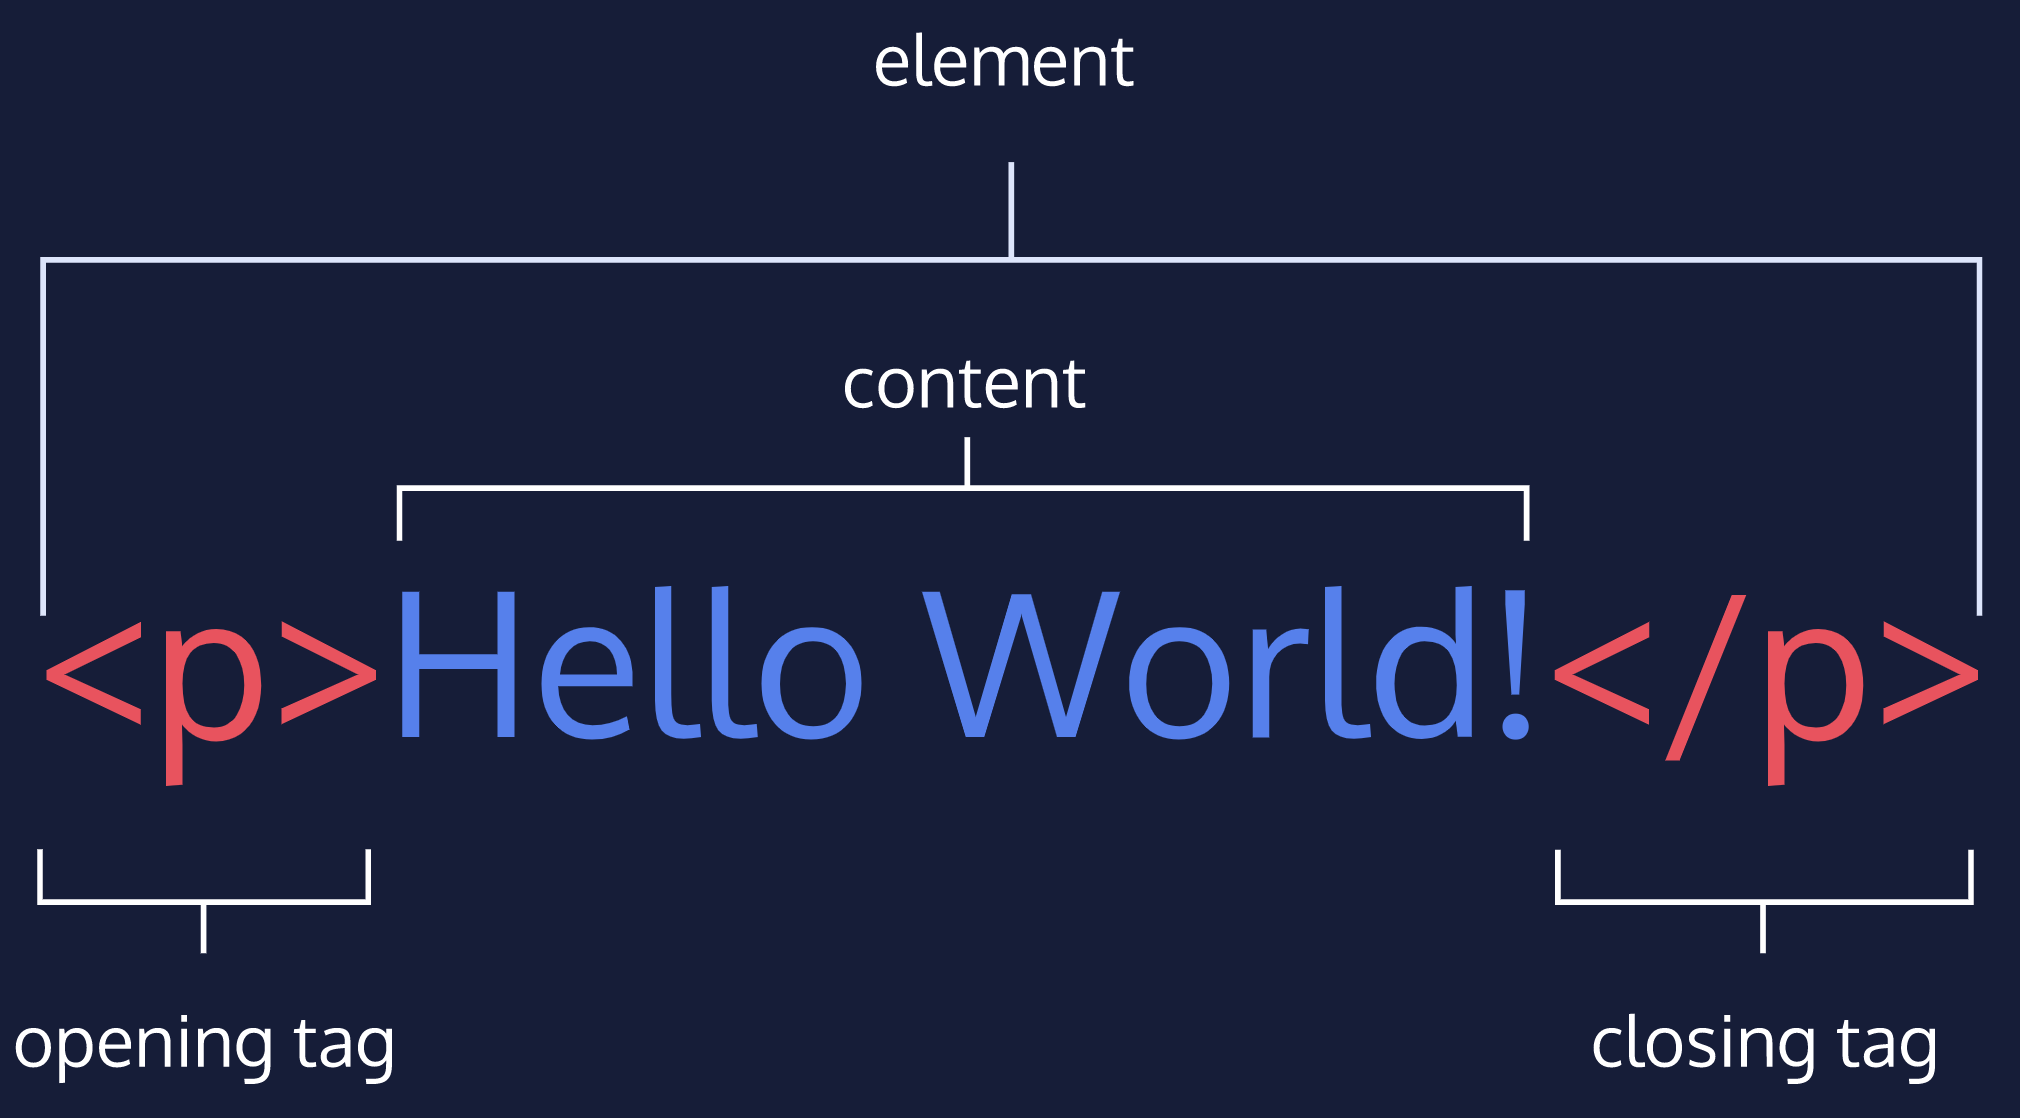
\includegraphics[scale = 0.2]{1_1}
\centering
\end{figure}
The diagram above displays an HTML paragraph element. As we can see, the paragraph element is made up of:
\begin{itemize}[leftmargin = *]
\item An \textit{opening tag} (\colorbox{lightgray}{<p>})
\item The content (“Hello World!” text)
\item A \textit{closing tag} (\colorbox{lightgray}{<$/$p>})
\end{itemize}
A \textit{tag} and the \textit{content} between it is called an HTML element. There are many tags that we can use to organize and display text and other types of content, like images. 

Let us quickly review each part of the element pictured:
\begin{itemize}[leftmargin = *]
\item HTML element (or simply, element) — a unit of content in an HTML document formed by HTML tags and the text or media it contains.
\item HTML Tag — the element name, surrounded by an opening (\colorbox{lightgray}{<}) and closing (\colorbox{lightgray}{>}) angle bracket. 
\item Opening Tag — the first HTML tag used to start an HTML element. The tag type is surrounded by opening and closing angle brackets.
\item Content — The information (text or other elements) contained between the opening and closing tags of an HTML element.
\item Closing tag — the second HTML tag used to end an HTML element. Closing tags have a forward slash (\colorbox{lightgray}{$/$}) inside of them, directly after the left angle bracket.
\end{itemize}

\subsection{The Body}
One of the key HTML elements we use to build a webpage is the \textit{body} element. Only content inside the opening and closing body tags can be displayed to the screen. Here is what opening and closing body tags look like:
\begin{lstlisting}
<body>

</body>
\end{lstlisting}
Once the file has a body, many different types of content – including text, images, and buttons – can be added to the body.
\begin{lstlisting}
<body>
  <p>What's up, doc?</p>
</body>
\end{lstlisting}

\subsection{HTML Structure}
HTML is organized as a collection of family tree relationships. As you saw in the last exercise, we placed \colorbox{lightgray}{<p>} tags within \colorbox{lightgray}{<body>} tags. When an element is contained inside another element, it is considered the \textit{child} of that element. The child element is said to be \textit{nested} inside of the \textit{parent} element.
\begin{lstlisting}
<body>
  <p>This paragraph is a child of the body</p>
</body>
\end{lstlisting}
In the example above, the \colorbox{lightgray}{<p>} element is nested inside the \colorbox{lightgray}{<body>} element. The \colorbox{lightgray}{<p>} element is considered a child of the \colorbox{lightgray}{<body>} element, and the \colorbox{lightgray}{<body>} element is considered the parent. Notice that we have added two spaces of indentation (using the \framebox[1.1\width]{space} bar) for better readability. 

Since there can be multiple levels of nesting, this analogy can be extended to grandchildren, great-grandchildren, and beyond. The relationship between elements and their ancestor and descendent elements is known as \textit{hierarchy}. 

Let us consider a more complicated example that uses some new tags: 
\begin{lstlisting}
<body>
  <div>
    <h1>Sibling to p, but also grandchild of body</h1>
    <p>Sibling to h1, but also grandchild of body</p>
  </div>
</body>
\end{lstlisting}
In this example, the \colorbox{lightgray}{<body>} element is the parent of the \colorbox{lightgray}{<div>} element. Both the \colorbox{lightgray}{<h1>} and \colorbox{lightgray}{<p>} elements are children of the \colorbox{lightgray}{<div>} element. Because the \colorbox{lightgray}{<h1>} and \colorbox{lightgray}{<p>} elements are at the same level, they are considered siblings and are both grandchildren of the \colorbox{lightgray}{<body>} element.

Understanding HTML hierarchy is important because child elements can inherit behavior and styling from their parent element. We will learn more about webpage hierarchy when you start digging into CSS.






\end{document}
